%%%%%%%%%%%%%%%%%%%%%%%%%%%%%%%%%%%%%%%%%%%%%%%%%%%%%%%%%%%%%%%%%%%%%%%%%%%%%%%%
%2345678901234567890123456789012345678901234567890123456789012345678901234567890
%        1         2         3         4         5         6         7         8

\documentclass[letterpaper, 10 pt, conference]{ieeeconf}  % Comment this line out if you need a4paper

%\documentclass[a4paper, 10pt, conference]{ieeeconf}      % Use this line for a4 paper

\IEEEoverridecommandlockouts                              % This command is only needed if 
                                                          % you want to use the \thanks command

\overrideIEEEmargins                                      % Needed to meet printer requirements.

%In case you encounter the following error:
%Error 1010 The PDF file may be corrupt (unable to open PDF file) OR
%Error 1000 An error occurred while parsing a contents stream. Unable to analyze the PDF file.
%This is a known problem with pdfLaTeX conversion filter. The file cannot be opened with acrobat reader
%Please use one of the alternatives below to circumvent this error by uncommenting one or the other
%\pdfobjcompresslevel=0
%\pdfminorversion=4

% See the \addtolength command later in the file to balance the column lengths
% on the last page of the document

% The following packages can be found on http:\\www.ctan.org
\usepackage{graphics} % for pdf, bitmapped graphics files
\usepackage{epsfig} % for postscript graphics files
\usepackage{mathptmx} % assumes new font selection scheme installed
\usepackage{times} % assumes new font selection scheme installed
\usepackage{amsmath} % assumes amsmath package installed
\usepackage{amsmath,amsfonts}
\usepackage{algorithmic}
\usepackage{algorithm}
\usepackage{array}
\usepackage[caption=false,font=normalsize,labelfont=sf,textfont=sf]{subfig}
\usepackage{textcomp}
\usepackage{stfloats}
\usepackage{url}
\usepackage{verbatim}
\usepackage{graphicx}
%\usepackage{amssymb}  % assumes amsmath package installed
\usepackage[style=ieee,backend=biber]{biblatex}
\addbibresource{ref.bib}

\title{\LARGE \bf
 MPPI Path Following with Foothold-Quality-Aware Cost for Quadruped Navigation in Unstructured Terrain*
}


\author{
% Muhammad Suleiman Qureshi$^{1}$ and Syeda Ailiya Fatima Rizvi$^{2}$% <-this % stops a space
\thanks{*This work was not supported by any organization}% <-this % stops a space
% \thanks{$^{1}$
%         {\tt\small mohammadsulaiman500@gmail.com}}%
% \thanks{$^{2}$
%         {\tt\small ailiya.fatima13@gmail.com}}%
}


\begin{document}



\maketitle
\thispagestyle{empty}
\pagestyle{empty}


%%%%%%%%%%%%%%%%%%%%%%%%%%%%%%%%%%%%%%%%%%%%%%%%%%%%%%%%%%%%%%%%%%%%%%%%%%%%%%%%
\begin{abstract}
Local planners used in mobile robot navigation evaluate trajectories based on center-of-mass collision checks, sufficient for wheeled platforms but inadequate for legged robots, whose stability depends on discrete foothold quality. We present a hierarchical framework that addresses this by augmenting a Model Predictive Path Integral (MPPI) local planner with a \textit{Foothold-Quality-Aware (FQA) critic}, which penalizes trajectories over unsteppable terrain, and a \textit{Turn-in-Place critic}, which suppresses destabilizing lateral motion. These are integrated with terrain-aware A* global planning and a convex centroidal MPC enhanced with slope-aligned friction cones, COM adaptation, and capture-point stepping. Ablation studies on a simulated Unitree Go2 in dense forest environments show that the full system achieves stable, fall-free traversal, while removing any component leads to significant degradation.
\end{abstract}


%%%%%%%%%%%%%%%%%%%%%%%%%%%%%%%%%%%%%%%%%%%%%%%%%%%%%%%%%%%%%%%%%%%%%%%%%%%%%%%%

\section{Introduction}

Autonomous quadruped robots possess an inherent structural advantage over wheeled vehicles in negotiating unstructured, hazardous, and uneven environments. By decoupling the body from the ground via articulated legs, quadrupeds can actively control their base posture, step over obstacles, and traverse discontinuous terrain such as forest floors, disaster sites, and rubble \cite{Hutter2016ANYmal, Bledt2018MITCheetah3}. However, unlocking this mobility requires a navigation stack capable of reasoning about the environment at multiple scales: from long-horizon global path planning down to high-frequency, contact-rich stabilizing leg control \cite{Fankhauser2018Robust}. 

The standard paradigm for autonomous navigation employs a hierarchical architecture. A global planner (e.g., A* or D* Lite) generates a collision-free path across a static grid, while a local planner such as the Dynamic Window Approach (DWA) or Model Predictive Path Integral (MPPI) control \cite{Williams2016Aggressive, Williams2016MPPI} computes reactive body-frame velocity commands to track the path and avoid unmapped dynamic obstacles. While heavily optimized for wheeled platforms (e.g., the ROS 2 Nav2 stack \cite{Macenski2023Nav2}), directly applying these local planners to legged robots introduces a significant gap: standard trajectory rollouts evaluate collisions and costs strictly based on the robot's Center of Mass (COM) footprint. 

For a wheeled robot, clearing the COM footprint is physically sufficient. For a quadruped, it is fundamentally inadequate. A quadruped's support polygon extends well beyond its body footprint. If a local planner commands the robot along a path where the COM is collision-free, but the required footholds lie on steep slopes, ridges, or deep gaps, the low-level locomotion controller will struggle to maintain contact stability, resulting in foot slippage, kinematic saturation, or catastrophic falls \cite{Kolter2009Stereo}.

Most contemporary solutions address this entirely at the low-level controller by employing terrain-aware heuristic foothold selection \cite{Mastalli2017Trajectory} or learning-based foothold adaptations \cite{Magana2019Fast, Miki2022Learning}. However, placing the burden of terrain negotiation solely on the reactive leg controller is suboptimal; if the local planner steers the robot into a region devoid of viable footholds, no amount of reactive adaptation can recover stability. A true solution requires the local path planner to be inherently \textit{locomotion-aware}.
\begin{figure}
    \centering
    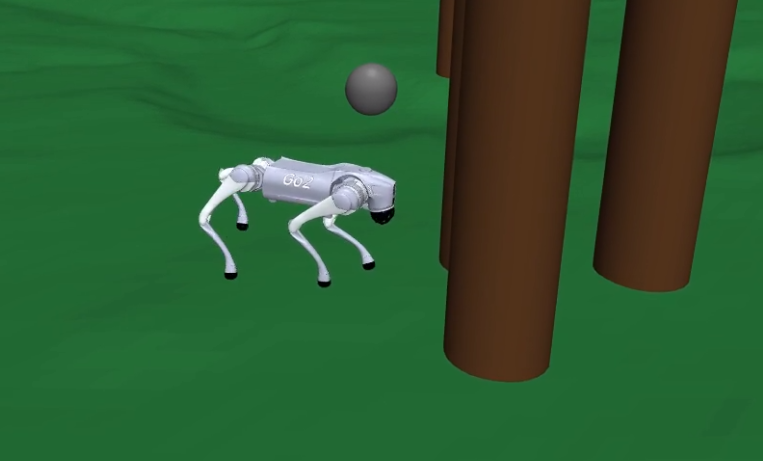
\includegraphics[width=0.85\linewidth]{go2.png}
    \caption{The Unitree go2 quadruped in a British Columbia forest pointcloud reconstructed on MuJoCo}
\end{figure}
In this paper, we propose a novel formulation of the MPPI local planner specifically designed for a quadruped robots  navigating unstructured forest-like terrain simulated on MuJoCo. Rather than evaluating costmaps via a monolithic COM footprint, we introduce a Foothold-Quality-Aware (FQA) critic that explicitly predicts the kinematics of all four legs along simulated rollouts, penalizing trajectories that require stepping on highly uneven or sloped surfaces. Furthermore, to address the destabilizing "crab-walking" (simultaneous forward and lateral motion) often observed when quadruped base velocities are commanded by omnidirectional planners, we introduce a Turn-in-Place critic that enforces stability-preserving heading alignment.

The specific contributions of this work are threefold:
\begin{enumerate}
    \item We introduce an FQA cost function for the MPPI planner that evaluates anticipated ground contact locations against a continuously derived terrain steppability map.
    \item We present a customized MPPI multi-critic architecture that actively suppresses unstable lateral quadruped kinematics by heavily penalizing large heading errors.
    \item We integrate these contributions into a complete, real-time hierarchical framework—combining perception, terrain-aware A*, MPPI, and a convex centroidal Model Predictive Controller (MPC)—and demonstrate its effectiveness in dense, unstructured simulated forest environments.
\end{enumerate}
\begin{figure*}[t]
\centering
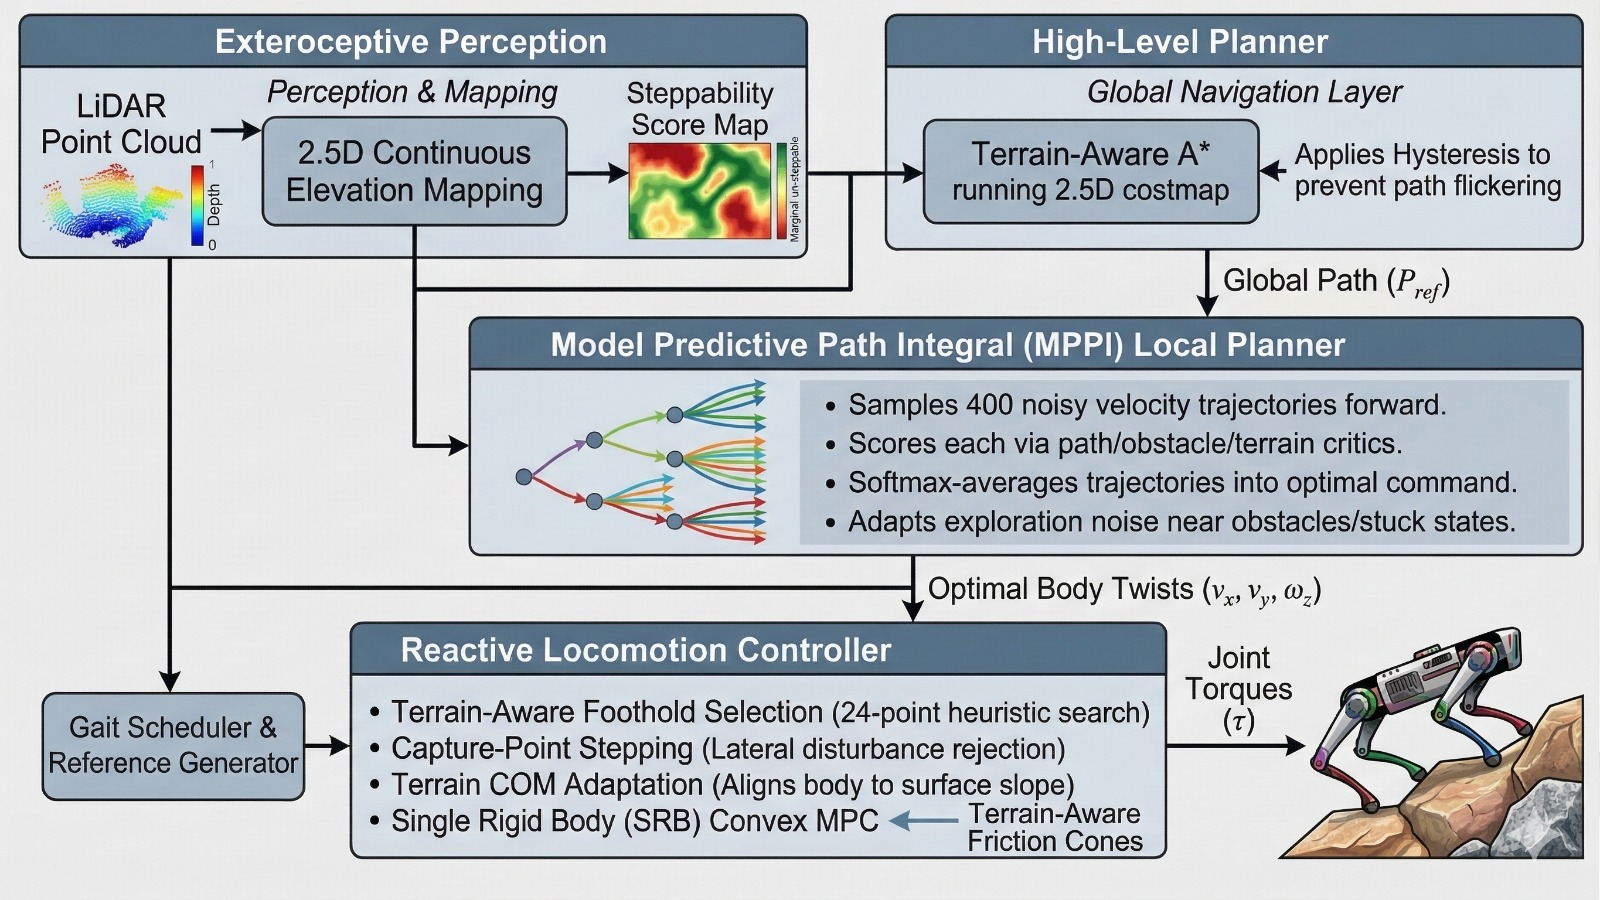
\includegraphics[width=0.77\textwidth]{image.png}
\caption{System architecture of the quadruped navigation framework.}
\label{fig:architecture}
\end{figure*}
The remainder of this paper is organized as follows. Section \ref{sec:related_work} reviews related work in quadruped navigation and sampling-based planning. Section \ref{sec:methodology} explicitly details the hierarchical architecture, the derivation of the FQA critic, and the low-level MPC tracking. Section \ref{sec:experiments} presents quantitative navigation metrics and qualitative behavior analysis, followed by ablation studies isolating the impact of our proposed critics in Section \ref{sec:ablation}. Section \ref{sec:conclusion} concludes the paper.


\section{Related Work}
\label{sec:related_work}
Model Predictive Control (MPC) has become the standard for highly dynamic quadruped locomotion, functioning effectively across varied terrain. Typically, these formulations employ Convex MPC based on simplified centroidal dynamics \cite{DiCarlo2018ConvexMPC} or tackle the full Whole-Body Nonlinear MPC \cite{Neunert2018WholeBodyNMPC} to account for explicit contact dynamics and kinematic constraints. While gradient-based methods excel at stabilizing continuous nonlinear dynamics, they struggle with severe non-convexities, such as discrete obstacle fields and discontinuous cost landscapes characteristic of rough terrain.

Recently, Model Predictive Path Integral (MPPI) control \cite{Williams2016MPPI} and generalized sampling-based MPC have gained traction in legged robotics to bypass gradient computation hurdles. Recent studies have demonstrated the deployment of whole-body sampling-based MPC on hardware \cite{Palo2024WholeBody}, highlighting its capacity to negotiate complex local minima without pre-defined contact schedules. Efforts to improve the sample efficiency of MPPI in locomotion have explored varied sampling distributions, such as spline-based action sequences \cite{Carius2026SamplingStrategies} and integration with Covariance Matrix Adaptation (CMA-ES) in the MPOPI framework \cite{Jiang2025MPOPI}. However, running MPPI at the low-level torque or contact force level remains computationally demanding for extended spatial horizons. In contrast to these whole-body sampling planners, our framework utilizes MPPI at the \textit{local navigation tier} operating in $SE(2)$, relying on standard Convex MPC for the low-level stabilization. This hierarchical split allows the MPPI planner to evaluate extensive spatial rollouts using terrain costmaps at high frequency.

To effectively utilize such terrain costmaps, selecting secure footholds is paramount for mitigating slip and ensuring stability on irregular topographies. Early frameworks combined geometric heuristics with search trees (e.g., A* or RRT*) to find kinematic plans over challenging obstacles, extensively demonstrated on platforms like LittleDog \cite{Kolter2008ControlArchitecture} and HyQ \cite{Winkler2014PathPlanning}. More recent methods quantify terrain desirability using dense 2.5D elevation maps. Fankhauser et al. \cite{Fankhauser2018Robust} demonstrated autonomous stair climbing on ANYmal using continuous elevation mapping, extracting surface normals and roughness to heuristically score footholds. Similarly, Mastalli et al. \cite{Mastalli2017Trajectory} jointly optimized CoM trajectories and footholds over terrain costmaps using CMA-ES, and Li et al. \cite{Li2019LearningCost} utilized Support Vector Machines (SVM) to learn foothold cost functions directly from expert demonstrations. Our work synergizes terrain evaluation directly into the continuous path generation layer. Rather than decoupling the path optimization from discrete footstep planning, our Foothold-Quality-Aware (FQA) critic continuously evaluates proposed SE(2) base trajectories by probabilistically sampling the underlying terrain quality where the robot's feet are predicted to land.

This integration of terrain-aware planning requires a robust system design. State-of-the-art quadruped stacks inherently rely on multi-layered architectures, decomposing the problem into global mapping, local trajectory planning, and high-frequency centroidal/whole-body control \cite{Hutter2016ANYmal,
Bledt2018MITCheetah3}. For autonomous navigation, these stacks frequently integrate variations of graph searches for global routes coupled with reactive local planners. In the broader mobile robotics domain, architectures like the ROS 2 Navigation stack (Nav2) employ MPPI controllers as well as local planners (e.g., DWB, TEB) that score velocity rollouts using footprint-based or 3D bounding box collision cost functions. Unfortunately, applying standard wheeled-robot critics to legged platforms drastically limits their mobility, as quadrupeds can actively step over obstacles that would obstruct a wheeled chassis. Our approach bridges the gap between conventional wheeled navigation and legged mobility by reformulating the MPPI local planner cost function. By scoring predicted discrete leg placements rather than treating the robot as a rigid footprint, the planner permits traversal over sparsely obstructed terrain. Furthermore, our architecture incorporates a turn-in-place (yaw) critic specifically tuned for quadrupeds, which penalizes lateral and diagonal velocity commands that risk displacing the center of mass into dynamically unstable configurations — reducing the likelihood of the characteristic 'crab-walk' singularities commonly induced by such commands in standard MPC tracking modules.

\section{Proposed Methodology}
\label{sec:methodology}
\subsection{System Overview}
The proposed framework decomposes autonomous quadruped navigation into four layers operating at distinct spatial and temporal scales (Fig. 1):
\begin{enumerate}
    \item \textbf{Global planning} (\ref{sec:astar}): A terrain-aware A* planner computes a collision-free waypoint path on a 2D cost grid at $\sim$12 Hz.
    \item \textbf{Local trajectory optimization} (\ref{sec:mppi}): An MPPI controller generates body-frame velocity commands $(v_x, v_y, \omega_z)$ that track the global path while satisfying legged-locomotion-specific costs, at $\sim$24 Hz.
    \item \textbf{Centroidal MPC} (\ref{sec:mpc}): A terrain-adaptive COM trajectory generator feeds a convex QP that resolves optimal ground reaction forces (GRFs) at $\sim$48 Hz, subject to terrain-aligned friction cone constraints.
    \item \textbf{Leg controller} (\ref{sec:leg_ctrl}): A per-leg task-space controller maps MPC forces to joint torques at 200 Hz, with distinct stance (force tracking) and swing (trajectory tracking) modes. A terrain-aware foothold selection heuristic with capture-point reactive stepping determines where each foot lands.
\end{enumerate}
The key insight motivating this hierarchy is that global planners reason over large spatial extents but use simplified collision models, while low-level controllers handle full rigid-body dynamics but have no notion of terrain quality beyond the immediate contact patch. The MPPI layer bridges this gap by evaluating candidate trajectories against \textit{leg-specific} terrain costs; the core contribution of this work. The steppability score $\sigma$ (\ref{eq:steppability}) is utilized at two levels: by the MPPI FQA critic to reject trajectories leading to poor-quality footholds, and by the low-level foothold selector to refine individual foot placements within the terrain that MPPI has pre-screened.
\subsection{Perception and Terrain Representation}
\subsubsection{Elevation Mapping}
A simulated 3D LiDAR ($N_{\text{az}} \times N_{\text{el}} = 90 \times 15 = 1350$ rays, $d_{\max} = 6$ m) generates point clouds that are accumulated into a fixed-frame elevation grid $\mathcal{G}$ of extent $W \times W = 12$ m $\times$ 12 m at resolution $\delta = 0.05$ m. Each cell $(i,j)$ maintains two height estimates updated via exponential moving average (EMA):
\begin{equation*}
h_g^{(i,j)} &\leftarrow (1 - \alpha_g)\, h_g^{(i,j)} + \alpha_g \cdot Q_{q_g}\!\left(\{z_k\}_{k \in (i,j)}\right)\\
\end{equation*}
\begin{equation*}
h_t^{(i,j)} &\leftarrow (1 - \alpha_t)\, h_t^{(i,j)} + \alpha_t \cdot \max\!\left(\{z_k\}_{k \in (i,j)}\right)
\end{equation*}

where $\alpha_g = 0.25$, $\alpha_t = 0.50$, $h_g$ is the ground layer ($q_g = 0.20$ quantile of observed heights, providing a robust walkable-surface estimate), and $h_t$ is the top layer (maximum observed height, capturing obstacle surfaces). The per-cell \textbf{clearance} $c^{(i,j)} = h_t^{(i,j)} - h_g^{(i,j)}$ distinguishes terrain variation from protruding obstacles.
\subsubsection{Steppability Score}
Drawing inspiration from continuous elevation mapping heuristics \cite{Fankhauser2018Robust, Mastalli2017Trajectory}, we define a continuous terrain quality metric $\sigma : \mathbb{R}^2 \to [0, 1]$ that combines two complementary indicators of foothold viability where the first term accounts for slope and the second for roughness:
\begin{equation}
\sigma(x, y) = w_s \cdot \min\!\left(\frac{\|\nabla h_g(x,y)\|}{s_{\max}}, 1\right) + w_r \cdot \min\!\left(\frac{\text{std}\!\left(h_g^{\mathcal{N}}\right)}{r_{\max}}, 1\right) \label{eq:steppability}
\end{equation}
with $w_s = 0.6$, $w_r = 0.4$, $s_{\max} = 0.5$ (gradient corresponding to $\approx 27^\circ$, near the friction limit for $\mu = 0.8$), and $r_{\max} = 0.03$ m. The gradient is computed via central finite differences and $\text{std}(\cdot)$ is evaluated over a 5-point cross-shaped neighbourhood $\mathcal{N}$. A score of $\sigma = 0$ denotes ideal flat ground; $\sigma = 1$ denotes untraversable terrain.
\subsubsection{Obstacle Cost Map}
Cells with clearance $c \geq c_{\text{lethal}} = 0.12$ m (the robot's step-over limit given a swing apex of 0.15 m) are classified as obstacles and inflated with a linearly decaying radial kernel of radius $r_{\text{inf}} = 0.50$ m:
\begin{equation}
\mathcal{C}_{\text{inf}}(d) = \mathcal{C}_{\text{raw}} \cdot \max\!\left(0,\; 1 - \frac{d}{r_{\text{inf}}}\right) \label{eq:inflation}
\end{equation}
The inflation radius accounts for the robot's half-width plus a dynamic tracking error margin.
\subsection{Terrain-Aware Global Planning}
\label{sec:astar}
\subsubsection{Weighted A* Formulation}
We compute global waypoints via weighted A* on the 8-connected cost grid $\mathcal{G}$. Let $\mathcal{C}(n)$ denote the obstacle costmap value and $\sigma(n)$ the steppability score at node $n$. The edge cost from node $n$ to neighbour $n'$ is:
\begin{multline}
g(n') = g(n) + \|\mathbf{p}_{n'} - \mathbf{p}_n\| \cdot \\
\left(1 + w_{\text{obs}}\!\left(e^{\beta\, \mathcal{C}(n')} - 1\right) + w_{\text{terr}} \cdot \sigma(n')\right) \label{eq:astar_edge}
\end{multline}
with $w_{\text{obs}} = 100$, $\beta = 4$, $w_{\text{terr}} = 5$. The \textbf{exponential obstacle penalty} creates a steep cost gradient that forces paths well into free space. At 50\% inflation ($\mathcal{C} = 0.5$), the multiplicative cost factor reaches $\approx 640\times$, effectively repelling paths from the inflation zone. The heuristic uses a $1.5\times$ Euclidean weight for faster search:
\begin{equation}
f(n) = g(n) + 1.5 \cdot \|\mathbf{p}_n - \mathbf{p}_{\text{goal}}\| \label{eq:heuristic}
\end{equation}
\subsubsection{Path Hysteresis}
To prevent oscillatory replanning around symmetric obstacle configurations, cells belonging to the previous path $\mathcal{P}_{t-1}$ receive a discounted traversal cost:
\begin{equation}
g_{\text{hyst}}(n') = \begin{cases} g(n') & \text{if } n' \notin \mathcal{P}_{t-1} \\ 0.5 \cdot g(n') & \text{if } n' \in \mathcal{P}_{t-1} \end{cases} \label{eq:hysteresis}
\end{equation}
The 50\% discount prevents topological oscillation (e.g., flipping between passing left vs. right of a tree) while permitting route changes if a newly discovered obstacle blocks the path. The raw path is then smoothed via constrained Laplacian smoothing to round corners without intersecting obstacles.
\subsection{Foothold-Quality-Aware MPPI}
\label{sec:mppi}
\subsubsection{MPPI Preliminaries}
We adopt the sampling-based MPPI framework \cite{Williams2016MPPI}. Define the state $\mathbf{s}_t = [x_t,\, y_t,\, \psi_t,\, v_{x,t},\, v_{y,t},\, \omega_{z,t}]^T \in \mathbb{R}^6$ and control $\mathbf{u}_t = [v_{x,\text{cmd}},\, v_{y,\text{cmd}},\, \omega_{z,\text{cmd}}]^T \in \mathcal{U}$ with bounds:
\begin{equation}
\mathcal{U} = \{v_x \in [-0.25, 0.75],\; v_y \in [-0.5, 0.5],\; \omega_z \in [-1.75, 1.75]\} \label{eq:bounds}
\end{equation}
The asymmetric $v_x$ bounds reflect gait stability constraints on the quadruped.
\subsubsection{Rollout Dynamics and Noise}
We propagate each rollout using a first-order velocity lag model that captures the response latency of the underlying centroidal MPC:
\begin{equation}
v_{x,t+1} = v_{x,t} + \frac{(v_{x,\text{cmd}} - v_{x,t})\,\Delta t}{\tau}, \qquad \tau = 0.4\,\text{s} \label{eq:lag}
\end{equation}
with analogous updates for $v_y$ and $\omega_z$. Position integration follows the standard unicycle model over $x$, $y$, and $\psi$. 
Candidate control sequences $\mathbf{U}_i$ are generated by perturbing the nominal sequence with temporally correlated AR(1) noise:
\begin{equation}
\boldsymbol{\epsilon}_{i,t} = \rho\,\boldsymbol{\epsilon}_{i,t-1} + (1-\rho)\,\boldsymbol{\eta}_{i,t}, \qquad \boldsymbol{\eta}_{i,t} \sim \mathcal{N}(\mathbf{0}, \boldsymbol{\Sigma}) \label{eq:ar1}
\end{equation}
with $\rho = 0.5$. Correlated noise produces feasible, arc-like trajectories rather than kinematically unrealisable zig-zag paths.
% \subsubsection{Turn-in-Place Critic (Crab-Walk Suppression)}
% When correcting path-following errors, quadrupeds commanded via body-frame velocity often exhibit simultaneous forward and lateral motion (``crab-walking''), which reduces the lateral stability margin. We introduce a critic that penalises forward velocity when the heading error $|\Delta\psi_t^{(i)}|$ is large:
% \begin{equation}
% C_{\text{turn}}^{(i)} = w_{\text{turn}} \frac{1}{H}\sum_{t=1}^{H} (v_{x,t}^{(i)})^2 \left[\max\!\left(0,\; |\Delta\psi_t^{(i)}| - \psi_{\text{dead}}\right)\right]^2 \label{eq:turn_critic}
% \end{equation}
% where $\psi_{\text{dead}} = 0.2$ rad ($\approx 11^\circ$). The quadratic coupling ensures the penalty is dominant for large heading errors. With $w_{\text{turn}} = 500$, the optimiser drops $v_x \to 0$ and uses $\omega_z$ to align the heading before moving forward.
% \subsubsection{Foothold-Quality-Aware (FQA) Critic}
% Standard MPPI evaluates trajectories by querying the costmap at the Center of Mass (COM) position. Because legged robots have distinct ground contact patches, we accurately predict where each foot will contact the ground during a rollout.
% Let $\mathbf{h}^l = (h_x^l, h_y^l)^T$ denote the body-frame hip offset for leg $l \in \{1,2,3,4\}$. The predicted world-frame foothold is:
% \begin{equation}
% \mathbf{f}^{l,t} = \begin{bmatrix} x^t \\ y^t \end{bmatrix} + \mathbf{R}_z(\psi^t)\,\mathbf{h}^l = \begin{bmatrix} x^t + h_x^l \cos\psi^t - h_y^l \sin\psi^t \\ y^t + h_x^l \sin\psi^t + h_y^l \cos\psi^t \end{bmatrix} \label{eq:foot_predict}
% \end{equation}
% The terrain steppability $\sigma$ from (\ref{eq:steppability}) is queried at each predicted foothold, and the FQA cost averages the squared penalty over all horizon steps $H$:
% \begin{equation}
% C_{\text{FQA}}^{(i)} = w_{\text{fqa}} \cdot \frac{1}{4H}\sum_{l=1}^{4}\sum_{t=1}^{H} \left[\sigma\!\left(\mathbf{f}^{l,t}\right)\right]^2 \label{eq:fqa_cost}
% \end{equation}
% The squared penalty cleanly amplifies the distinction between mediocre and severely poor footholds, guaranteeing that MPPI avoids paths requiring steps across untraversable terrain.
% The total cost aggregates standard Nav2 terms (Path-Follow, Path-Progress, Obstacle Clearance) alongside FQA ($w_{\text{fqa}} = 3.0$) and Turn-in-Place.
\subsubsection{Multi-Critic Cost Function}
Each candidate trajectory $i$ incurs a total cost $C_i$ that is the sum of eight critic terms. We detail the two novel critics below, followed by a summary of all terms.
\begin{itemize}
    \item \textbf{Turn-in-Place Critic (Crab-Walk Suppression):} When correcting path-following errors, quadrupeds commanded via body-frame velocity often exhibit simultaneous forward and lateral motion (``crab-walking''), which reduces the lateral stability margin. We introduce a critic that penalises forward velocity when the heading error $|\Delta\psi_t^{(i)}|$ is large:
    \begin{equation}
    C_{\text{turn}}^{(i)} = w_{\text{turn}} \frac{1}{H}\sum_{t=1}^{H} [\max(0, v_{x,t}^{(i)})]^2 \left[\max\!\left(0,\; |\Delta\psi_t^{(i)}| - \psi_{\text{dead}}\right)\right]^2 \label{eq:turn_critic}
    \end{equation}
    where $\psi_{\text{dead}} = 0.2$ rad ($\approx 11^\circ$). The quadratic coupling ensures the penalty is dominant for large heading errors. With $w_{\text{turn}} = 500$, the optimiser drops $v_x \to 0$ and uses $\omega_z$ to align the heading before moving forward.\\
    
    \item \textbf{Foothold-Quality-Aware (FQA) Critic:} Standard MPPI \cite{Williams2016MPPI} evaluates trajectories by querying the costmap at the Center of Mass (COM) position. Because legged robots have distinct ground contact patches, we accurately predict where each foot will contact the ground during a rollout, shifting the terrain evaluation from discrete footstep planners \cite{Kolter2008ControlArchitecture, Winkler2014PathPlanning, Li2019LearningCost} directly into the continuous trajectory rollout.
    
    Let $\mathbf{h}^l = (h_x^l, h_y^l)^T$ denote the body-frame hip offset for leg $l \in \{1,\dots,4\}$. The predicted world-frame foothold is:
    \begin{equation}
    \mathbf{f}^{l,t} = \begin{bmatrix} x^t \\ y^t \end{bmatrix} + \mathbf{R}_z(\psi^t)\,\mathbf{h}^l = \begin{bmatrix} x^t + h_x^l \cos\psi^t - h_y^l \sin\psi^t \\ y^t + h_x^l \sin\psi^t + h_y^l \cos\psi^t \end{bmatrix} \label{eq:foot_predict}
    \end{equation}
    Note: this assumes zero capture-point displacement, i.e., feet land directly below the hip. This is a valid approximation at low forward speeds where the Raibert velocity-dependent offset $\mathbf{v} \cdot T_{\text{stance}}/2$ is small relative to the hip spread. \\
    The terrain steppability $\sigma$ from (\ref{eq:steppability}) is queried at each predicted foothold, and the FQA cost averages the squared penalty over all horizon steps $H$:
    \begin{equation}
    C_{\text{FQA}}^{(i)} = w_{\text{fqa}} \cdot \frac{1}{4H}\sum_{l=1}^{4}\sum_{t=1}^{H} \left[\sigma\!\left(\mathbf{f}^{l,t}\right)\right]^2 \label{eq:fqa_cost}
    \end{equation}
    The squared penalty cleanly amplifies the distinction between mediocre and severely poor footholds, guaranteeing that MPPI avoids paths requiring steps across untraversable terrain.
\end{itemize}
\
The total cost aggregates standard Nav2 terms (Path-Follow, Path-Progress, Obstacle Clearance) alongside FQA ($w_{\text{fqa}} = 3.0$) and Turn-in-Place. Table \ref{tab:critics} summarizes all terms.
\begin{table}[ht]
\centering
\caption{Complete MPPI Critic Formulation}
\label{tab:critics}
\begin{tabular}{|p{1.25cm}|p{0.75cm}|p{5.05cm}|}
\hline
\textbf{Critic} & \textbf{Weight $w$} & \textbf{Cost Definition} \\
\hline
Path-follow & 80 & Mean cross-track distance to A* path \\
Path-angle & 120 & Mean $|\psi_t - \text{atan2}(\Delta p_y, \Delta p_x)|$ \\
Turn-in-place & 500 & Eq. (\ref{eq:turn_critic}): $v_x^2 \cdot \max(0, |\Delta\psi| - 0.2)^2$ \\
Path-progress & 20 & $(L - s_{\max})/L$; penalises lack of advance \\
Obstacle & 30--300 & Graduated: 300 (lethal), $150\mathcal{C}$ (mod.), $30\mathcal{C}$ (mild) \\
Slope & 2.5 & Mean $\|\nabla h_g\|$ along trajectory \\
\textbf{FQA} & \textbf{3.0} & \textbf{Eq. (\ref{eq:fqa_cost}): Squared steppability at feet} \\
Smoothness & 0.1 & Mean $\|\Delta \mathbf{u}_t\|$ (control rate penalty) \\
\hline
\end{tabular}
\end{table}
\subsubsection{Optimal Control via Softmax Weighting}
The optimal control sequence $\mathbf{U}^*$ is computed as the information-theoretic weighted average:
\begin{equation}
\mathbf{U}^* = \sum_{i=1}^{K} w_i\, \mathbf{U}_i, \qquad w_i \propto \exp\!\left(-\frac{C_i - C_{\min}}{\lambda}\right) \label{eq:softmax}
\end{equation}
with inverse temperature $\lambda = 8.0$. After $N_{\text{iter}}=5$ optimization iterations, the first step of the control sequence is extracted, rate-limited, and passed to the low-level controller.
\subsection{Centroidal MPC and Low-Level Control}
\label{sec:mpc}

\subsubsection{Terrain-Adaptive COM Trajectory}
\label{sec:com_adapt}
Before solving the centroidal QP, the reference trajectory $\mathbf{x}_k^{\text{ref}}$ must account for the terrain beneath the robot. Rather than commanding a fixed body height and level orientation, we generate terrain-consistent references along the prediction horizon:

\textbf{Height adaptation.} At each horizon step $k$, the reference COM height is set relative to the local ground level:
\begin{equation}
z_k^{\text{ref}} = \max\!\left(z_{\text{terrain}}(x_k, y_k),\; \bar{z}_{\text{hips},k}\right) + h_{\text{nom}} \label{eq:com_height}
\end{equation}
where $z_{\text{terrain}}(\cdot)$ is the ground height queried from the elevation map at the predicted COM position, $\bar{z}_{\text{hips},k}$ is the mean terrain height sampled at the four projected hip locations, and $h_{\text{nom}} = 0.27$ m is the nominal standing height. Taking the maximum prevents body sagging when the COM passes over a local depression while the feet remain on higher surrounding terrain.

\textbf{Orientation alignment.} The roll and pitch references are lightly blended toward the terrain surface normal $\hat{\mathbf{n}} = (n_x, n_y, n_z)^T$ queried at each horizon step:
\begin{equation}
\phi_k^{\text{ref}} = \alpha_{\text{slope}} \cdot \arctan\!\left(\frac{-n_y}{n_z}\right), \quad \theta_k^{\text{ref}} = \alpha_{\text{slope}} \cdot \arctan\!\left(\frac{n_x}{n_z}\right) \label{eq:com_rpy}
\end{equation}
with blending factor $\alpha_{\text{slope}} = 0.25$. Full alignment ($\alpha = 1$) would sacrifice the gyroscopic stability benefits of an upright torso; partial alignment reduces the gravitational moment arms acting on the legs and keeps joint positions near the center of their workspace. The vertical velocity reference $\dot{z}_k^{\text{ref}}$ is derived via finite differences of the terrain-adjusted height trajectory, providing the QP with a smooth $z$-tracking target over slopes.

\subsubsection{QP Formulation}
The body-frame velocity commands $(v_x^*, v_y^*, \omega_z^*)$ from MPPI are combined with the terrain-adaptive COM trajectory to form the full reference $\mathbf{x}_k^{\text{ref}}$. We model the quadruped using Single Rigid Body (SRB) dynamics \cite{DiCarlo2018ConvexMPC} and optimize ground reaction forces (GRFs) across a 16-step horizon (equivalent to one full $0.33$~s trot cycle). This is formulated as a sparse Quadratic Program (QP):
\begin{equation}
\min_{\mathbf{X}, \mathbf{U}} \sum_{k=0}^{N-1} \left[(\mathbf{x}_k - \mathbf{x}_k^{\text{ref}})^T \mathbf{Q}\,(\mathbf{x}_k - \mathbf{x}_k^{\text{ref}}) + \mathbf{u}_k^T \mathbf{R}\,\mathbf{u}_k\right] \label{eq:qp_objective}
\end{equation}
Here, the state vector $\mathbf{x}_k \in \mathbb{R}^{12}$ tracks the robot's base position, orientation (roll, pitch, yaw), linear, and angular velocities. The control vector $\mathbf{u}_k \in \mathbb{R}^{12}$ comprises the 3D forces at each stance foot. To ensure gait stability, the tracking error cost $\mathbf{Q}$ heavily penalizes deviations in body height ($q_z=50$) and pitch/roll ($q_{\theta}=20, q_{\phi}=10$), while lateral $x,y$ position tracking is left loose ($q_x=q_y=1$) since the MPPI layer handles spatial path guidance. The $\mathbf{R}$ matrix serves purely as a Hessian regularizer ($\mathbf{R}=10^{-5}\mathbf{I}$).

\subsubsection{Terrain-Adaptive Friction Constraints}
The QP enforces friction pyramid limits ($\mu = 0.8$) to ensure the feet do not slip. On sloping terrain, friction cones aligned to world-gravity become physically invalid. To counter this, the contact surface normal $\hat{\mathbf{n}}$ at each leg's predicted touchdown location is queried from the height map. A local tangent basis $(\mathbf{t}_1, \mathbf{t}_2, \hat{\mathbf{n}})$ is constructed, and the four friction pyramid faces are expressed as:
\begin{equation}
\pm\mathbf{t}_j^T \mathbf{f} \leq \mu\, \hat{\mathbf{n}}^T \mathbf{f}, \quad j \in \{1,2\} \label{eq:friction_cone}
\end{equation}
with an additional minimum normal force constraint $\hat{\mathbf{n}}^T \mathbf{f} \geq f_{\min} = 10$ N to prevent lift-off during stance. This rotation is applied per-leg, per-timestep, allowing the QP to reason about heterogeneous contact surfaces (e.g., one foot on flat ground, another on a 20$^\circ$ slope).

\subsubsection{Leg Controller}
\label{sec:leg_ctrl}
The MPC outputs optimal GRFs $\mathbf{f}^l_{\text{mpc}}$ for each stance leg $l$. A per-leg task-space controller running at 200 Hz maps these to joint torques, with distinct modes for stance and swing:

\textbf{Stance phase.} The MPC contact force is mapped to joint torques via the foot Jacobian transpose, augmented with a foothold-hold PD controller that resists foot sliding:
\begin{equation}
\boldsymbol{\tau}_{\text{stance}} = \mathbf{J}_l^T \left(-\mathbf{f}^l_{\text{mpc}} + \mathbf{K}_p^{\text{st}} \mathbf{e}_{p} + \mathbf{K}_d^{\text{st}} \mathbf{e}_{v}\right) + \left(\mathbf{C}\dot{\mathbf{q}} + \mathbf{g}\right)_l \label{eq:stance_tau}
\end{equation}
where $\mathbf{e}_p = \mathbf{p}_{\text{td}} - \mathbf{p}_{\text{foot}}$ is the position error relative to the recorded touchdown point, $\mathbf{K}_p^{\text{st}} = \text{diag}(300, 300, 0)$, $\mathbf{K}_d^{\text{st}} = \text{diag}(40, 40, 20)$, and $(\mathbf{C}\dot{\mathbf{q}} + \mathbf{g})_l$ compensates Coriolis and gravitational torques for the leg joints.

\textbf{Swing phase.} An operational-space inverse dynamics controller tracks the desired swing trajectory:
\begin{equation}
\boldsymbol{\tau}_{\text{swing}} = \mathbf{J}_l^T \left(\mathbf{K}_p^{\text{sw}} \mathbf{e}_p + \mathbf{K}_d^{\text{sw}} \mathbf{e}_v + \boldsymbol{\Lambda}_l(\ddot{\mathbf{x}}_{\text{des}} - \dot{\mathbf{J}}_l \dot{\mathbf{q}})\right) + \left(\mathbf{C}\dot{\mathbf{q}} + \mathbf{g}\right)_l \label{eq:swing_tau}
\end{equation}
where $\boldsymbol{\Lambda}_l = (\mathbf{J}_l \mathbf{M}^{-1} \mathbf{J}_l^T)^{-1}$ is the operational-space inertia matrix, $\mathbf{K}_p^{\text{sw}} = 400\mathbf{I}_3$,  and $\mathbf{K}_d^{\text{sw}} = 75\mathbf{I}_3$. The feedforward term $\boldsymbol{\Lambda}_l(\ddot{\mathbf{x}}_{\text{des}} - \dot{\mathbf{J}}_l\dot{\mathbf{q}})$ compensates for the foot's acceleration requirements and Jacobian rate effects, enabling precise trajectory tracking through a minimum-jerk swing profile with apex height 0.15 m.

\subsubsection{Terrain-Aware Foothold Selection}
\label{sec:foothold_sel}
At each swing-leg takeoff, the nominal touchdown position is computed via the Raibert heuristic with velocity and position feedback. This nominal is then refined by evaluating $K = 24$ candidate footholds sampled in structured concentric rings (1 center, 8 inner at $0.5r$, 12 outer at $r$, 3 forward-biased; $r = 0.15$ m) around the nominal, rotated into the walking direction.

Candidates are first filtered by hard gates: maximum surface slope ($25^\circ$), kinematic reachability ($0.08 \leq d_{\text{hip}} \leq 0.35$ m), vertical jump limit ($|\Delta z| \leq 0.10$ m), plane-fit residual ($\leq 0.015$ m RMS, rejecting edges and holes), and COM stability margin (the predicted COM must lie inside the support polygon at touchdown). Surviving candidates are scored by a weighted sum of six normalized soft terms:
\begin{equation}
S = w_{\text{stab}}\, \hat{s}_{\text{stab}} + w_{\text{dist}}\, \hat{s}_{\text{dist}} + w_{\text{slope}}\, \hat{s}_{\text{slope}} + w_{\text{res}}\, \hat{s}_{\text{res}} + w_{\text{spd}}\, \hat{s}_{\text{spd}} + w_{\text{grade}}\, \hat{s}_{\text{grade}} \label{eq:foothold_score}
\end{equation}
where each $\hat{s}$ is min-max normalized to $[0,1]$. The terms and their baseline weights are listed in Table \ref{tab:foothold_weights}.

\begin{table}[ht]
\centering
\caption{Foothold Selection Scoring Criteria}
\label{tab:foothold_weights}
\begin{tabular}{|p{1.1cm}|p{0.55cm}|p{5.4cm}|}
\hline
\textbf{Term} & \textbf{$w$} & \textbf{Description} \\
\hline
Stability & 0.20 & Support-polygon margin: distance from predicted COM to nearest edge of the convex hull of stance contacts. Larger margin $\to$ lower penalty. \\
Distance & 0.25 & Deviation from Raibert nominal; penalizes large corrections. \\
Slope & 0.20 & Local surface inclination at foothold. \\
Residual & 0.20 & Plane-fit RMS over a $12\times12$ cm patch; measures local curvature and edge proximity. \\
Speed & 0.10 & Forward-progress bias along walking direction. \\
Grade & 0.05 & Terrain grade preference: front legs favor uphill, rear legs favor downhill to maintain pitch stability. \\
\hline
\end{tabular}
\end{table}

Critically, the stability weight $w_{\text{stab}}$ is \textit{adaptive}: it is boosted from its baseline of 0.20 up to 0.70 as a function of roll severity:
\begin{equation}
w_{\text{stab}} = 0.20 + 0.50 \cdot \min\!\left(1,\; \frac{|\phi|}{10^\circ} + \frac{|\dot{\phi}|}{1\,\text{rad/s}}\right) \label{eq:adaptive_stab}
\end{equation}
where $\phi$ is the body roll angle and $\dot{\phi}$ the roll rate. When the robot is rolling, the selector automatically prioritizes widening the support polygon over minimizing deviation from the nominal foothold.

\subsubsection{Capture-Point Reactive Stepping}
\label{sec:capture_point}
The foothold selector alone optimizes over a static set of candidates. To handle dynamic lateral disturbances (e.g., a sudden slope-induced roll), we augment the Raibert nominal with a capture-point offset before candidate evaluation. Modeling the robot as a linear inverted pendulum with natural frequency $\omega_0 = \sqrt{g/h_{\text{nom}}} \approx 6.0$ rad/s, the lateral capture displacement in the body frame is:
\begin{equation}
p_{\text{cap},y} = \frac{v_{\text{lat}}}{\omega_0} - \sin(\phi) \cdot h_{\text{nom}} \label{eq:capture_point}
\end{equation}
where $v_{\text{lat}}$ is the lateral COM velocity in the body frame and $\phi$ is the roll angle. When the capture point falls on the same side as the current swing leg (e.g., the robot is falling rightward and the right leg is swinging), the nominal is shifted laterally by $0.6 \cdot p_{\text{cap},y}$ in world coordinates, effectively widening the stance to catch the falling COM. The 0.6$\times$ gain prevents overshoot.

\subsubsection{MPPI--MPC--Leg Controller Synergy}
The FQA critic acts as a spatial pre-filter: MPPI actively penalizes COM trajectories that place peripheral legs into terrain with high steppability scores, so the reference velocities passed to the MPC natively guide the robot through clustered safe zones. The terrain-adaptive COM trajectory ensures the QP tracks physically consistent height and orientation references. The terrain-aligned friction cones guarantee force feasibility on slopes. The foothold selector, operating within terrain pre-screened by MPPI, only needs to perform local refinement among nearby candidates rather than global search. This layered synergy---where each component narrows the problem space for the layer below---is key to the system's robustness, as validated by the ablation study (Section~\ref{sec:ablation}).

%%%%%%%%%%%%%%%%%%%%%%%%%%%%%%%%%%%%%%%%%%%%%%%%%%%%%%%%%%%%%%%%%%%%%%%%%%%%%%%%

\section{Experimental Results}

The robot traverses 5m from (-2,0) to (3,0) across 5 LiDAR-derived terrains from British Columbia forests, each with randomized obstacles: 15 tree trunks (cylinders), 3 rocks (spheres), and 2 fallen logs (capsules) — placed to block the direct path and force the planner to find detours. Positions are rejection-sampled to keep start/goal areas clear. The simulation duration is 20 secs on a randomized terrain.

Traversal time reports how long the robot took to reach within 0.75m of the goal. Body contacts counts collisions between the robot's body (excluding feet) and obstacles, indicating whether the robot physically struck any object or fell during navigation. Roll (deg) measures the mean absolute lateral body tilt during traversal, reflecting locomotion stability over uneven terrain.
\begin{figure}
    \centering
    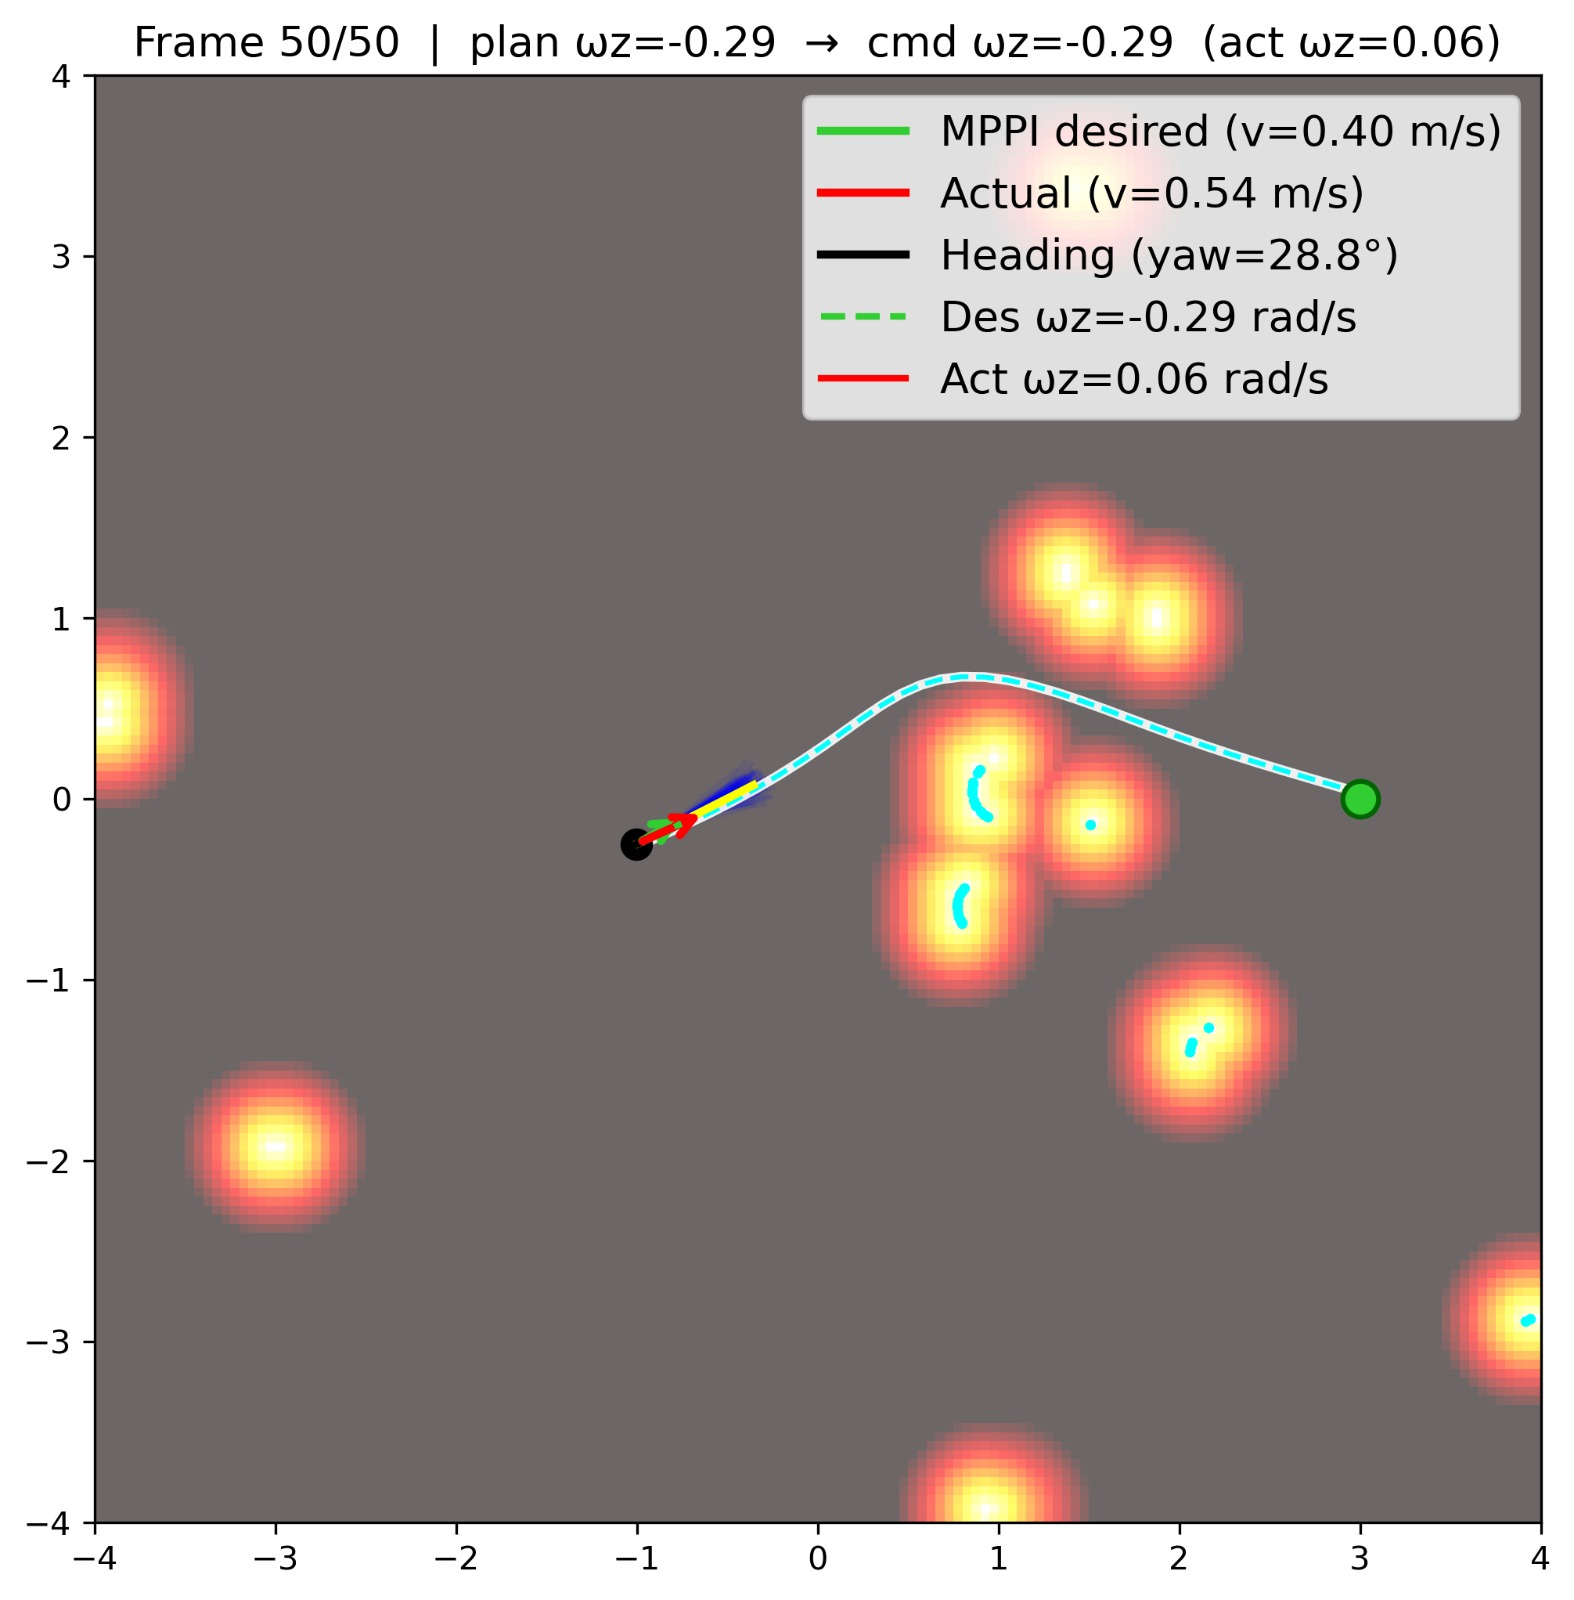
\includegraphics[width=0.75\linewidth]{mppi.png}
    \caption{Example frame from the MPPI-based local planner operating in a cluttered environment. The planner generates a smooth trajectory (cyan dashed line) toward the goal (green marker) while avoiding obstacles represented by the costmap heatmap. The green arrow denotes the desired velocity from MPPI, the red arrow shows the robot's actual velocity, and the black arrow indicates the current heading. The planner commands an angular velocity of −0.29 rad/s, while the measured yaw rate is 0.06 rad/s.}
\end{figure}
This tests generalization of the convex MPC + MPPI planner across varied terrain and obstacle layouts.
\label{sec:experiments}
\begin{table}[h]
\centering
\begin{tabular}{lccccc}
\hline
\textbf{Environment} & \textbf{Time (s)} & \textbf{Roll (deg)}& \textbf{Contacts}\\
\hline
bc\_094p006\_2\_2\_3\_xli1m\_utm10 & 14.7 & 12.5 & 0 \\
bc\_083e021\_xli1m\_utm11\_2019 & 12.5 & 9.19 & 0  \\
bc\_093f077\_xli1m\_utm10\_2019  & 18.0 & 9.62 & 0  \\
bc\_093f097\_xli1m\_utm10\_2019  & 16.9 & 8.79 & 0  \\
bc\_093g045\_xli1m\_utm10\_2019  & 16.2 & 7.63 & 0  \\
\hline
\end{tabular}
\caption{Results across Five British Columbia LiDAR-derived terrain environments.\cite{BC}}
\label{tab:environments}
\end{table}
\section{Ablation Study}
\label{sec:ablation}

To systematically evaluate the contribution of each proposed component within our hierarchical navigation framework, we conducted a comprehensive ablation study. The experiments involve navigating a simulated Go2 quadruped over a challenging 5-meter unstructured terrain course (from $x = -2$ m to $x = 3$ m) with obstacles on a single hand-tuned scene. Each trial has a maximum duration of 18 seconds. The primary metrics for evaluation are: success rate (Goal Reached), final distance to the goal, Roll/Pitch Root Mean Square (RMS) to quantify stability, and the total number of body contacts (falls). 

The results of the ablation study are summarized in Table \ref{tab:ablation_results}. We compare the full proposed system (Baseline) against seven degraded configurations, each with a specific feature disabled.

\begin{table*}[!t]
\centering
\caption{Ablation Study Results: 5m Traversal over Uneven Terrain}
\label{tab:ablation_results}
\resizebox{\textwidth}{!}{%
\begin{tabular}{l c c c c c}
\toprule
\textbf{Configuration} & \textbf{Goal Reached} & \textbf{Final Dist. (m)} & \textbf{Roll RMS (rad)} & \textbf{Pitch RMS (rad)} & \textbf{Body Contacts} \\
\midrule
\textbf{Case 0: Full System (Baseline)} & \textbf{Yes (14.7s)} & \textbf{0.23} & \textbf{0.27} & \textbf{0.07} & \textbf{0} \\
Case 1: No Path Planning & No & 2.65 & 0.12 & 0.05 & 0 \\
Case 2: No FQA Steppability Critic & No & 2.54 & 0.89 & 0.13 & 4 \\
Case 3: No Terrain Friction Cones & Yes (15.8s) & 0.42 & 0.36 & 0.18 & 6 \\
Case 4: No Terrain COM Adaptation & Yes (17.9s) & 0.72 & 0.73 & 0.16 & 8 \\
Case 5: No Capture-Point Stepping & No & 2.46 & 0.87 & 0.28 & 12 \\
Case 6: No Terrain Foothold Selection & No & 1.23 & 0.72 & 0.11 & 7 \\
Case 7: Blind Locomotion & No & 1.76 & 1.83 & 0.17 & 9 \\
\bottomrule
\end{tabular}%
}
\end{table*}

\subsection{Analysis of Ablations}

\textbf{Case 0: Full System (Baseline).} The complete framework successfully reaches the goal in 14.7 seconds with a final distance of 0.23 m. It maintains a low Roll RMS (0.27 rad, or 15.5$^\circ$) and, crucially, achieves zero body contacts. This is the only configuration that demonstrates clean, stable traversal without any falls, establishing the baseline performance of the integrated system.

\textbf{Case 1: No Path Planning.} Disabling the MPPI planner forces the robot to rely on a naive goal-seeking heuristic (direct heading). While the robot remains stable (Roll RMS of 0.12 rad, zero falls), it gets stuck behind obstacles, failing to reach the goal (2.65 m remaining). The total path length is only 4.16 m compared to the baseline's 8.34 m. This demonstrates that while local stability is maintained by the low-level controller, high-level path planning is essential for navigating around complex obstacles and avoiding dead ends.

\textbf{Case 2: No FQA Steppability Critic.} Removing the Foothold-Quality-Aware (FQA) critic from the MPPI cost function allows the planner to select paths traversing geometrically feasible but dynamically unstable terrain (e.g., steep slopes or sharp edges). The robot fails to reach the goal, Roll RMS spikes to 0.89 rad (max roll 180$^\circ$), and the robot suffers 4 body contacts. This highlights the critical role of the FQA critic in preventing the planner from guiding the robot into unsteppable terrain regions.

\textbf{Case 3: No Terrain Friction Cones.} When the MPC assumes flat-ground friction cones rather than adapting to the local surface normal, the robot reaches the goal but suffers significant performance degradation (15.8 seconds, 0.42 m final distance). Roll RMS increases to 0.36 rad, and the robot incurs 6 body contacts. The MPC commands forces that violate actual friction limits on slopes, causing slippage and partial falls. Terrain-aware friction cones are thus vital for force feasibility and reliable slope climbing.

\textbf{Case 4: No Terrain COM Adaptation.} Disabling both terrain-aware COM height and orientation adjustments forces the robot to maintain a level body posture regardless of the underlying slope. The robot reaches the goal, but does so slowly (17.9 seconds) and with the worst performance among successful cases. Roll RMS reaches 0.73 rad, max roll hits 180$^\circ$, and the robot suffers 8 body contacts. Fighting the terrain creates large moment arms and forces legs to their kinematic limits, proving that COM adaptation is crucial for maintaining workspace limits and balance.

\textbf{Case 5: No Capture-Point Stepping.} Disabling capture-point stepping (lateral foot widening during roll) and adaptive stability weighting removes the robot's primary reactive balance mechanism against lateral disturbances. The robot fails to reach the goal, with a Roll RMS of 0.87 rad and a total of 12 body contacts across 72 steps—the highest fall count of any ablation. Without capture-point stepping to catch the shifting Center of Mass, any disturbance quickly cascades into a catastrophic fall, making this the single most important feature for maintaining reactive balance on rough terrain.

\textbf{Case 6: No Terrain Foothold Selection.} Disabling both terrain-aware foothold selection (evaluating candidates based on slope, stability, and planarity) and the MPPI steppability critic forces the robot to step at nominal Raibert heuristic positions. The robot fails to reach the goal (1.23 m remaining), suffering 7 body contacts with a Roll RMS of 0.72 rad. Although the robot makes significant forward progress, indiscriminate foot placement on edges and unstable patches causes repeated stumbling. 

\textbf{Case 7: Blind Locomotion.} Disabling all terrain-aware features—leaving only LiDAR-based obstacle detection—results in near-total failure. The robot fails to reach the goal, experiencing continuous tumbling with a Roll RMS of 1.83 rad (mean 92$^\circ$) and 9 body contacts. The simulation terminates early due to continuous failure to recover. This catastrophic degradation validates the necessity of the proposed hierarchical approach: terrain perception and reactive adaptation are not optional enhancements, but fundamental requirements for legged locomotion in unstructured environments.

\subsection{Summary of Contributions}
The ablation results reveal a clear functional hierarchy within the proposed framework. Reactive balance mechanisms (capture-point stepping, foothold selection) are the primary defense against falls. Perception-informed path planning (MPPI, FQA critic) ensures the robot chooses dynamically viable routes, avoiding geometrically feasible but unstable terrain. Finally, terrain-aware centroidal dynamics (friction cones, COM adaptation) optimize force distribution and maintain kinematic reachability. Removing any single layer significantly degrades performance, and removing all layers (Case 7) results in total failure, affirming the necessity of the integrated system design.

\section{Conclusion and Future Work}
\label{sec:conclusion}

In this paper, we presented a hierarchical navigation architecture for quadruped robots that explicitly bridges the gap between high-level path planning and low-level reactive locomotion. By integrating a Foothold-Quality-Aware (FQA) critic and a Turn-in-Place critic into a Model Predictive Path Integral (MPPI) local planner, the framework ensures that generated velocity commands adhere to the terrain's steppability constraints and preserve the robot's lateral stability margin. Coupled with a terrain-aware centroidal Model Predictive Controller (MPC) and reactive foothold adaptation mechanisms, our approach significantly reduces the frequency of catastrophic falls on unstructured terrain. Extensive ablation studies in simulated dense forest environments validated that removing any component of this perception-to-control pipeline drastically degrades locomotor performance, demonstrating that intelligent path planning and reactive balance are fundamentally codependent for robust legged navigation.

Despite the promising results demonstrated in simulations, several avenues remain open for future research. First, we aim to conduct more robust testing across a wider variety of extreme environments, including but not limited to stairs, sheer drop-offs, cliffs, and dynamic moving obstacles, to further evaluate the framework's operational limits. 

Second, we plan to deeply integrate exteroceptive vision (e.g., RGB or semantic cameras) directly into the costmap generation process. This will enable semantic reasoning about physical surface properties—such as estimating terrain friction coefficients before stepping, or identifying non-geometric hazards like water, ice, and mud—which LiDAR-based elevation maps inherently cannot detect.

Thirdly, incorporating adaptive gait scheduling based on the navigation difficulty of the terrain and the desired traversal speed represents a crucial next step. For example, the system could autonomously transition to a highly stable, albeit slower, crawl gait when navigating treacherous, high-cost regions, while automatically shifting to a dynamic trot to maximize speed and efficiency across flatter ground. 

Most critically, we plan to deploy the framework on a physical Unitree Go2. A successful sim-to-real transfer will primarily require integrating a robust onboard localization pipeline (e.g., LiDAR-inertial odometry), as the current system relies on ground-truth pose available only in simulation, along with careful compensation for actuator delays and sensor noise.
%%%%%%%%%%%%%%%%%%%%%%%%%%%%%%%%%%%%%%%%%%%%%%%%%%%%%%%%%%%%%%%%%%%%%%%%%%%%%%%%




% \begin{thebibliography}{99}

% \bibitem{c1} G. O. Young, ÒSynthetic structure of industrial plastics (Book style with paper title and editor),Ó 	in Plastics, 2nd ed. vol. 3, J. Peters, Ed.  New York: McGraw-Hill, 1964, pp. 15Ð64.
% \bibitem{c2} W.-K. Chen, Linear Networks and Systems (Book style).	Belmont, CA: Wadsworth, 1993, pp. 123Ð135.
% \bibitem{c3} H. Poor, An Introduction to Signal Detection and Estimation.   New York: Springer-Verlag, 1985, ch. 4.
% \bibitem{c4} B. Smith, ÒAn approach to graphs of linear forms (Unpublished work style),Ó unpublished.
% \bibitem{c5} E. H. Miller, ÒA note on reflector arrays (Periodical styleÑAccepted for publication),Ó IEEE Trans. Antennas Propagat., to be publised.
% \bibitem{c6} J. Wang, ÒFundamentals of erbium-doped fiber amplifiers arrays (Periodical styleÑSubmitted for publication),Ó IEEE J. Quantum Electron., submitted for publication.
% \bibitem{c7} C. J. Kaufman, Rocky Mountain Research Lab., Boulder, CO, private communication, May 1995.
% \bibitem{c8} Y. Yorozu, M. Hirano, K. Oka, and Y. Tagawa, ÒElectron spectroscopy studies on magneto-optical media and plastic substrate interfaces(Translation Journals style),Ó IEEE Transl. J. Magn.Jpn., vol. 2, Aug. 1987, pp. 740Ð741 [Dig. 9th Annu. Conf. Magnetics Japan, 1982, p. 301].
% \bibitem{c9} M. Young, The Techincal Writers Handbook.  Mill Valley, CA: University Science, 1989.
% \bibitem{c10} J. U. Duncombe, ÒInfrared navigationÑPart I: An assessment of feasibility (Periodical style),Ó IEEE Trans. Electron Devices, vol. ED-11, pp. 34Ð39, Jan. 1959.
% \bibitem{c11} S. Chen, B. Mulgrew, and P. M. Grant, ÒA clustering technique for digital communications channel equalization using radial basis function networks,Ó IEEE Trans. Neural Networks, vol. 4, pp. 570Ð578, July 1993.
% \bibitem{c12} R. W. Lucky, ÒAutomatic equalization for digital communication,Ó Bell Syst. Tech. J., vol. 44, no. 4, pp. 547Ð588, Apr. 1965.
% \bibitem{c13} S. P. Bingulac, ÒOn the compatibility of adaptive controllers (Published Conference Proceedings style),Ó in Proc. 4th Annu. Allerton Conf. Circuits and Systems Theory, New York, 1994, pp. 8Ð16.
% \bibitem{c14} G. R. Faulhaber, ÒDesign of service systems with priority reservation,Ó in Conf. Rec. 1995 IEEE Int. Conf. Communications, pp. 3Ð8.
% \bibitem{c15} W. D. Doyle, ÒMagnetization reversal in films with biaxial anisotropy,Ó in 1987 Proc. INTERMAG Conf., pp. 2.2-1Ð2.2-6.
% \bibitem{c16} G. W. Juette and L. E. Zeffanella, ÒRadio noise currents n short sections on bundle conductors (Presented Conference Paper style),Ó presented at the IEEE Summer power Meeting, Dallas, TX, June 22Ð27, 1990, Paper 90 SM 690-0 PWRS.
% \bibitem{c17} J. G. Kreifeldt, ÒAn analysis of surface-detected EMG as an amplitude-modulated noise,Ó presented at the 1989 Int. Conf. Medicine and Biological Engineering, Chicago, IL.
% \bibitem{c18} J. Williams, ÒNarrow-band analyzer (Thesis or Dissertation style),Ó Ph.D. dissertation, Dept. Elect. Eng., Harvard Univ., Cambridge, MA, 1993. 
% \bibitem{c19} N. Kawasaki, ÒParametric study of thermal and chemical nonequilibrium nozzle flow,Ó M.S. thesis, Dept. Electron. Eng., Osaka Univ., Osaka, Japan, 1993.
% \bibitem{c20} J. P. Wilkinson, ÒNonlinear resonant circuit devices (Patent style),Ó U.S. Patent 3 624 12, July 16, 1990. 


\printbibliography
% \vspace{1em}
% Fix IEEEbiography photo alignment to top
% \makeatletter
% \let\old@IEEEbiography\@IEEEbiography
% \renewenvironment{IEEEbiography}[2][]{\old@IEEEbiography[#1]{#2}\vspace{0pt}}{}
% \makeatother
% \begin{IEEEbiography}[{
\includegraphics[width=1in,height=1.25in,clip,keepaspectratio]{black.png}}]{IEEE Publications Technology Team}
% In this paragraph you can place your educational, professional background and research and other interests.\end{IEEEbiography}
\vspace{2em}
\noindent\begin{minipage}[t]{\columnwidth}
  \begin{minipage}[t]{1in}
    \vspace{0pt}
    
\includegraphics[width=1in,height=1.25in,clip,keepaspectratio]{black.png}
  \end{minipage}%
  \hspace{0.2in}%
  \begin{minipage}[t]{\dimexpr\columnwidth-1in-0.2in\relax}
    \vspace{0pt}
    {\bfseries Suleiman Qureshi} is currently pursuing research in autonomous
    quadrupedal locomotion and terrain-aware navigation using model predictive
    control and sampling-based planners. His interests include hierarchical
    control architectures, real-time motion planning.
  \end{minipage}
\end{minipage}
\vspace{2em}
\\
\noindent\begin{minipage}[t]{\columnwidth}
  \begin{minipage}[t]{1in}
    \vspace{0pt}
    
\includegraphics[width=1in,height=1.25in,clip,keepaspectratio]{black.png}
  \end{minipage}%
  \hspace{0.2in}%
  \begin{minipage}[t]{\dimexpr\columnwidth-1in-0.2in\relax}
    \vspace{0pt}
    {\bfseries Ailiya Fatima} is currently pursuing research in autonomous
    quadrupedal locomotion and terrain-aware navigation using model predictive
    control and sampling-based planners. His interests include hierarchical
    control architectures, real-time motion planning, and sim-to-real transfer
    for legged robots.
  \end{minipage}

\end{minipage}

% \vspace{1em}
% \noindent\begin{minipage}[t]{\columnwidth}
%   \begin{minipage}[t]{1in}
%     \vspace{0pt}
%     
\includegraphics[width=1in,height=1.25in,clip,keepaspectratio]{black.png}
%   \end{minipage}%
%   \hspace{0.15in}%
%   \begin{minipage}[t]{\columnwidth-1.15in}
%     \vspace{0pt}
%     {\bfseries Ailiya Fatima} works on perception-driven locomotion systems
%     and robotic navigation in unstructured environments. Her research focuses
%     on terrain mapping, sensor fusion, and autonomous navigation frameworks
%     for mobile robots.
%   \end{minipage}
% \end{minipage}
% \begin{IEEEbiography}[{
\includegraphics[width=1in,height=1.25in,clip,keepaspectratio]{black.png}}]{Suleiman Qureshi}
% \vspace{-34pt}is currently pursuing research...
% \end{IEEEbiography}

% \begin{IEEEbiography}[{
\includegraphics[width=1in,height=1.25in,clip,keepaspectratio]{black.png}}]{Ailiya Fatima}
% \vspace{-34pt}works on perception-driven locomotion...
% \end{IEEEbiography}

% \begin{IEEEbiography}[{
\includegraphics[width=1in,height=1.25in,clip,keepaspectratio]{black.png}}]{Suleiman Qureshi}
% \vspace{-16pt}is currently pursuing research in autonomous quadrupedal locomotion 
% and terrain-aware navigation using model predictive control and sampling-based planners.
% His interests include hierarchical control architectures, real-time motion planning,
% and sim-to-real transfer for legged robots.
% \end{IEEEbiography}
% \\

% \\
% \begin{IEEEbiography}[{
\includegraphics[width=1in,height=1.25in,clip,keepaspectratio]{black.png}}]{Ailiya Fatima}
% works on perception-driven locomotion systems and robotic navigation 
% in unstructured environments. Her research focuses on terrain mapping,
% sensor fusion, and autonomous navigation frameworks for mobile robots.
% \end{IEEEbiography}
% \begin{IEEEbiography}[{\fbox{\rule{0pt}{1.25in}\rule{1in}{0pt}}}]{Ailiya Fatima}

% \end{IEEEbiography}



% \end{thebibliography}




\end{document}
